
\documentclass[xcolor=dvipsnames]{beamer}
\usepackage[]{bnumexpr}
\usepackage{outlines}
\usepackage{multimedia}
\usepackage{pgffor}
\usetheme{Frankfurt}

\title{Fractal Automata}
\subtitle{Using Fractal Neural Networks to Play SimCity 1 and Conway's Game of Life at Variable Scales}

\author{Sam Earle}
%\institute{Bedroom Coder}
\date{\today}
\usepackage{array,graphicx}
\usepackage{pgfplots}
\usepackage{tikz}
\usepackage{amsmath}
\usepgfplotslibrary{groupplots}
\usepackage{adjustbox}
\usepackage{animate}
\usetikzlibrary{arrows}
\usetikzlibrary{matrix}
\usetikzlibrary{positioning}

\definecolor{ao}{rgb}{0.0, 0.0, 1.0}
\definecolor{amber}{rgb}{1.0, 0.49, 0.0}
\definecolor{ao green}{rgb}{0.0, 0.5, 0.0}
\definecolor{americanrose}{rgb}{1.0, 0.01, 0.24}
\definecolor{amethyst}{rgb}{0.6, 0.4, 0.8}
\definecolor{auburn}{rgb}{0.43, 0.21, 0.1}

\pgfplotsset{compat=newest}
\begin{document}

\begin{frame}
\titlepage
\end{frame}

\begin{frame}
\frametitle{Outline}
\tableofcontents
\end{frame}
	\section{Introduction}
\begin{frame}
	Goal: to have an A.I. play SimCity.
\end{frame}
\begin{frame}
	Approach:
	\begin{itemize}
		\item observation: 2D image of map, channels of tilestates
		\item action: 2D image of map, channels of (tile-specific) actions
		\item agent observes map, takes one tile-specific action, city sim ticks, repeat
		\item agent is rewarded for population (or some combination of city-wide metrics) once per step
	\end{itemize}

	Desiderata: 
	\begin{outline}
			\1 an agent should be able to play the game on various map-sizes
			\1 an observation in one corner of the map can affect an action taken in the opposite corner
    Non-athropomorphic agents invite new metaphors.
    \end{outline}
\end{frame}
\begin{frame}
	What does `expert play' look like in the context of an open-ended simulation?
	\begin{outline}
			\1 to transfer gracefully between interesting states
			\1 to achieve simulation-states with varying global characteristics by effective combinations of local actions, e.g.:
			\2 \textit{Roller Coaster Tycoon's} scenarios (num. guests, park/roller-coaster rating, cash flow, etc.)
            \2 player-generated goals in \textit{The Sims} (e.g., new couple in town conspires to drown entire neighbourhood in ladderless pool; player engaging in high-level games not represented directly by the software itself)

	\end{outline}

	In addition to an overall score, we have other global metrics like cash flow, population by zone-type, traffic, crime rate, citizen happiness, land value, etc.
\end{frame}
\begin{frame}
	Goal: to have an A.I. play SimCity, or, to extend SimCity with A.I.
	\begin{outline}
			\1 to extend the human player's abilities and knowledge
				\2 abilities: e.g., `build a low-density residential neighbourhood in the 2nd quadrant of the map'
				\2 knowledge: i.e., indirectly, as the player witnesses the layout-strategies used to achieve various goals, gaining new insight into simulation logic % Casual Content Creator
	\end{outline}
	Auxiliary goal: develop RL-agent extension for Geographical Information Software (GIS)
	\begin{outline}
		\1 Planners specify global (or local) constraints, agent drafts multiple possible city layouts. % Insert ethical concerns here
	\end{outline}
\end{frame}
\section{Environments}
\subsection{Micropolis}
\begin{frame}
	\frametitle{Micropolis}
	The player builds  power plants, zones, services, and infrastructure on a 2D grid, to attract residential, commercial and industrial development. Traffic results. The player has to manage the emergent global dynamics of localized forces to keep the city alive.

\begin{center}
       \animategraphics[autoplay,loop,width=0.490\linewidth]{30}{gifs/boredom-}{0}{200} 
\end{center}
	

\end{frame}
\begin{frame}
	\frametitle{Simulation Quirks}
	 	\animategraphics[autoplay,loop,width=0.490\linewidth]{30}{gifs/trafficQuirk-}{0}{200} 
	 	\animategraphics[autoplay,loop,width=0.490\linewidth]{30}{gifs/trafficQuirk2-}{0}{200}
\end{frame}
\begin{frame}
	Circuitous commutes.
	\begin{outline}
			\1 In SC4, visible traffic is produced by a collection of CA's, and ``only loosely'' influenced by pathfinding algorithms. From the guide to the Network Addon Mod (NAM) mod for SimCity4, which extends the traffic simulator:
			\end{outline}
				\begin{quote}
					To a very large extent, then, the traffic simulator is actually a desirability generator.
				\end{quote}
				\begin{quote}
					\dots the destination finder has been tuned aggressively by Maxis in ways that we cannot access in order to minimize how much the pathfinder must run, since finding paths is one of the most expensive operations (in terms of CPU time and memory) in SC4.
\end{quote}
\begin{outline}
\1 Idea: implement traffic simulator as stack of pathfinding CA and send to GPU for parallel processing.
\2 Train randomly initialized stack of CA as NN, in pytorch, to imitate NAM-like, CPU-based traffic sim.
\end{outline}

\end{frame}
\begin{frame}
	\begin{columns}
		\begin{column}{0.3\textwidth}
			Agent learns to avoid traffic, which is repellant and unnecessary, by limiting connectivity of networks.
			\linebreak

			\includegraphics[width=\linewidth]{images/resQuirk.png}
			{\small
			Above: agent-inspired utopian hack
			Right: (NIMBY)-human and agent collaboration
		}
		\end{column}
		\begin{column}{0.7\textwidth}
			\animategraphics[autoplay,loop,width=\linewidth]{30}{gifs/resHack-}{0}{200}
		\end{column}
	\end{columns}
\end{frame}
%\begin{frame}
%    Rewarding traffic has weird consequences.
%    \animategraphics[autoplay,loop,width=.6\linewidth]{30}{gifs/collab-}{0}{1700}
%\end{frame}
\begin{frame}
    Local strategies scale more easily than global ones.
    \includegraphics[width=\linewidth]{images/frac_intra_MP_builds.png}
\end{frame}
\begin{frame}
    \includegraphics[width=\linewidth]{images/traffic_upfail.png}
\end{frame}
\begin{frame}
	First observation: spatial logic is preserved at multiple scales.
	\begin{outline}
		\1 traffic flows between neighbourhoods, cities, and regions; so do power, trash, and goods
			\2 model with repeated convolutions		
		\1 specialized subregions exert forces of desirability and demand at multiple scales
			\2 model with convolutions applied to variable-size maps.
\end{outline}
	Consider possible subtask of predicting power flow over grid.
    \begin{outline}
        \1 Use a CA: "if I am not an obstacle, and I am adjacent to a powered cell, then I am a powered cell"
            \2 Can easily implement this with a single repeated convolution and a (hard) tanh activation.
    \end{outline}
\end{frame}
\begin{frame}
Batty and Longley, 1994, show that fractals can be used to generate plausible urban plans, and that real cities have fractal dimension.
\begin{columns}
    \begin{column}{0.5\linewidth}
        \includegraphics[width=\linewidth]{images/cardiffSim.png}
    \end{column}
    \begin{column}{0.5\linewidth}
        \includegraphics[width=\linewidth]{images/cardiffReal.png}
    \end{column}
\end{columns}
\end{frame}
\begin{frame}
    \begin{columns}
        \begin{column}{0.4\linewidth}
            \includegraphics[width=\linewidth]{images/idealizedCAurban.png}
            \includegraphics[width=\linewidth]{images/stochCAurban.png}
        \end{column}
        \begin{column}{0.6\linewidth}
    Batty, 1997, shows that Cellular Automata can be used to create idealized and stochastic fractal urban geometries.
            \includegraphics[width=\linewidth]{images/mixCAurban.png}
        \end{column}
    \end{columns}
\end{frame}
\begin{frame}
    Local zoning strategies lead to emergent neighbourhoods at various scales.
    \includegraphics[width=\linewidth]{big_ded.jpeg}
\end{frame}
\subsection{Game of Life}
\begin{frame}
	\frametitle{Conway's Game of Life}
	A 2D binary grid is (uniformly) randomly initialized. Based on (spatially-invariant) rules about neighbouring cells, the state of each cell at $t_i + 1$ is computed in parallel. A rich variety of global dynamics may result.
	For RL:
	\begin{itemize}
		\item After each tick of the simulation, a player/agent can activate a single cell. 
		\item Agent is rewarded for net active-cell count (i.e., population)
	\end{itemize}
    \begin{columns}
        \begin{column}{0.5\linewidth}
            \animategraphics[autoplay,loop,width=0.490\linewidth]{30}{gifs/vanillaGoL-}{0}{220} 
        \end{column}
        \begin{column}{0.5\linewidth}
            \animategraphics[autoplay,loop,width=0.490\linewidth]{30}{gifs/agentGoL-}{0}{220} 
        \end{column}
    \end{columns}
\end{frame}
\begin{frame}
    \includegraphics[width=\linewidth]{images/frac_intra_GoL_builds.png}
    \includegraphics[width=\linewidth]{GoL.png}
\end{frame}
\begin{frame}
    \frametitle{Game of Life: Qualitative Observations}
    \begin{outline}
        \1 All agents tend to build branching, stable structure, usually only once the simulation has reached a near-static state.
            \2 Hard to tell if the agents actively quell chaos, or simply wait for dust to settle.
            \2 In rare cases, though, agents that learn to build stable structures on small maps, have a different experience on larger ones: a cloud of oscillating chaos gradually fills the board, then stabilizes.
        \1 Agents sometimes get caught in oscillators, or participate in glider-like structures.

    \end{outline}
\end{frame}
\subsection{Power Puzzle}
\begin{frame}
\frametitle{Power Puzzle}
A random micropolis map is initialized, with one power plant and multiple residential zones. The agent must deliver power to each, as quickly as possible (to achieve maximum population reward per episode).
\begin{outline}
\1 Per-step reward demands \textit{time-sensitive} spanning tree, which adds nodes to tree using shortest available path, s.t. (num. powered zones) / (num. timesteps) is maximized.
\end{outline}
\end{frame}
\begin{frame}
    \begin{columns}
        \begin{column}{0.5\linewidth}
    \includegraphics[width=\linewidth]{images/PP_20.png}
        \end{column}
        \begin{column}{0.5\linewidth}
    \includegraphics[width=\linewidth]{images/PP_64.png}
        \end{column}
    \end{columns}
\end{frame}
\begin{frame}
       \animategraphics[autoplay,loop,width=0.8\linewidth]{30}{gifs/casual-}{0}{100} 
\end{frame}
%\begin{frame}
%      \animategraphics[autoplay,loop,width=0.490\linewidth]{30}{gifs/entomb-}{0}{200} 
%\end{frame}
\section{Methods}
\begin{frame}
    \frametitle{Learning Algorithm}
	In Advantage Actor Critic (A2C), the agent must produce an action and a scalar value-prediction at each step. The value prediction is trained to predict the `return' of a given map-state, which is a function of the reward it generates, while the action prediction is trained to optimize the predicted value of the resulting map-state.
	\begin{itemize}
		\item To allow 2D input and output of variable dimensions, stick to convolutional layers.
		\item To generate the value-prediction, recursively apply a single strided convolution shrinking the hidden 2D activation as necessary.
\end{itemize}
\end{frame}
\begin{frame}
    \frametitle{Network Architecture}
    \begin{columns}
        \begin{column}{0.6\linewidth}

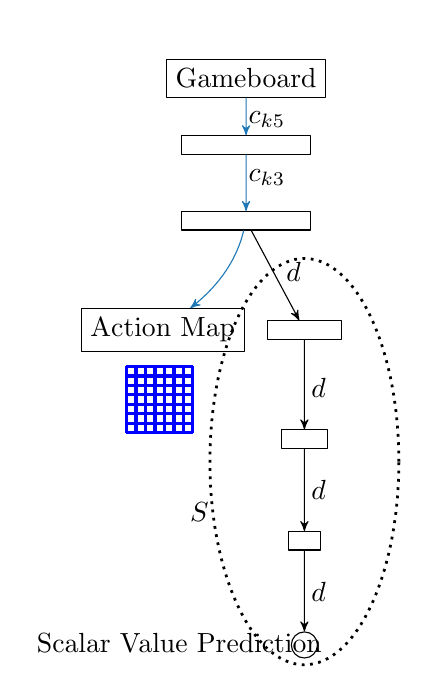
\begin{tikzpicture}[>=latex',line join=bevel,scale=0.6]
%%
\node (A) at (100.0bp,360bp) [draw,rectangle] {Gameboard};
\node (B) at (100.0bp,320bp) [draw,rectangle] {\hspace*{40pt}$$};
  \node (C) at (100.0bp,274.5bp) [draw,rectangle] {\hspace*{40pt}$$};
  \node (D) at (50.0bp,209.0bp) [draw,rectangle] {Action Map};
  \node (E) at (135.0bp,209.0bp) [draw,rectangle] {\hspace*{20pt}};
  \node (F) at (135.0bp,143.5bp) [draw,rectangle] {\hspace*{10pt}};
  \node (G) at (135.0bp,82.5bp) [draw,rectangle] {\hspace*{5pt}$$};
  \draw[dotted, line width=1] (135bp, 130bp) ellipse (2cm and 4.3cm);
  \node (H) at (135.0bp,20.0bp) [draw,circle] {$$};
  \definecolor{strokecolor}{rgb}{0.12,0.47,0.71};
  \draw [strokecolor,-stealth'] (A) -> (B);
  \definecolor{strokecol}{rgb}{0.0,0.0,0.0};
  \pgfsetstrokecolor{strokecol}
  \draw (112.5bp,335bp) node { $c_{k5}$};
  \draw (94.0bp,384.83bp) node {$$};
  \draw (94.0bp,344.21bp) node {$$};
  \definecolor{strokecolor}{rgb}{0.12,0.47,0.71};
  \draw [strokecolor,-stealth'] (B) -> (C);
  \draw (112.5bp,300.5bp) node { $c_{k3}$};
  \draw (94.0bp,324.93bp) node {$$};
  \draw (94.0bp,284.28bp) node {$$};
  \definecolor{strokecolor}{rgb}{0.12,0.47,0.71};
  \draw [strokecolor,-stealth'] (C) ..controls (97.155bp,262.85bp) and (92.141bp,242.33bp)  .. (D);
  \definecolor{strokecolor}{rgb}{0,0,0};
  \draw [strokecolor,-stealth'] (C) ..controls (106.77bp,261.83bp) and (120.07bp,236.94bp)  .. (E);
  \draw (128.5bp,244.0bp) node {$d$};
  \draw (95.882bp,264.98bp) node {$$};
  \draw (127.11bp,218.54bp) node {$$};
  \draw [strokecolor,-stealth'] (E) ..controls (135.0bp,196.59bp) and (135.0bp,172.88bp)  .. (F);
  \draw (143.5bp,174.0bp) node {$d$};
  \draw (129.0bp,199.48bp) node {$$};
  \draw (129.0bp,153.04bp) node {$$};
  \draw [strokecolor,-stealth'] (F) ..controls (135.0bp,131.46bp) and (135.0bp,110.28bp)  .. (G);
  \draw (143.5bp,113.0bp) node {$d$};
  \draw (129.0bp,133.87bp) node {$$};
  \draw (129.0bp,92.038bp) node {$$};
  \draw [strokecolor,-stealth'] (G) ..controls (135.0bp,70.483bp) and (135.0bp,50.078bp)  .. (H);
  \draw (143.5bp,52.0bp) node {$d$};
  \draw (129.0bp,72.778bp) node {$$};
  \draw (129.0bp,31.325bp) node {$$};
  \draw (72bp,100.0bp) node {$S$};
  \draw (60bp,21.0bp) node {Scalar Value Prediction};
  \draw [step=0.2,blue, very thick] (.99,5.19) grid (2.4,6.6);

%
\end{tikzpicture}
        \end{column}
        \begin{column}{0.4\linewidth}
            In order to calculate a scalar value prediction regardless of map size, replace the fully-connected layer in Vinyals, 2017 with a (variably) repeated, strided convolution.
        \end{column}
    \end{columns}
\end{frame}
\newcount\nodewidth
\nodewidth=48
\newcount\ncols
	\tikzset{equal/.style={draw, dotted, very thick, CadetBlue}}
	\tikzset{joinlayer/.style={draw, dashed, very thick}}
	\tikzset{down/.style={draw, ->, BrickRed ,very thick}}
	\tikzset{up/.style={draw, ->, OliveGreen, very thick}}
	\tikzset{conv/.style={draw, ->, very thick}}
	\tikzset{convlabel/.style={anchor=west,inner sep=5, color=black}}
	\tikzset{hidden/.style={rectangle, draw, minimum width=1cm, align=center, fill=gray, 
	fill opacity=0.1}}
	\tikzset{legendtext/.style={anchor=west,inner sep=10, color=black, text height=0.1mm}}
\begin{figure}
\newcommand{\xscale}{1}
\newcommand{\yscale}{3}
\begin{tikzpicture}[scale=0.8]
\matrix[at={(1.3,-2.2)}, minimum height=1, anchor=north west, font=\footnotesize]{
\draw[conv] (0,0) -- node[legendtext] {Convolution $f$} (0.6,0);& \\
\node [hidden, label=right: ($32\times32$) Activation Map] {};\\
%\node [hidden, minimum width=\nodewidth/2, fill opacity=0.4, align=center, label=right: ($16\times16$) ''] at (12pt, 0){};  \\
%\node [hidden, minimum width=\nodewidth/4, fill opacity=1,label=right:($8\times 8$) ''] at (18pt, 0){}; \\
\draw[joinlayer] (0,0) -- node[legendtext] {Join Operation (el.-wise averaging)} (0.6,0);\\
\draw[equal] (0,0) -- node[legendtext] {Equality} (0.6,0);\\
};

\newcommand{\coli}{black}
\gdef\fracnet#1#2#3#4{
    \edef\col{\number\numexpr#1\relax}%a+b
    \edef\dep{\number\numexpr#2}%a+b
    \edef\ypos{\number\numexpr#3\relax}
    \edef\incol{\number\numexpr\ncols-\col\relax}%a+b
    \edef\subcolh{\bnumexpr2^(\col)\relax}
    \edef\maxdepth{\bnumexpr2^(\ncols-1)\relax}
    \edef\coldepth{\bnumexpr\number2^(\ncols-\number\col)\relax}
    \edef\yposI{\number\numexpr\ypos+\bnethe\subcolh\relax}
    \edef\yposO{\number\numexpr\ypos-\bnethe\subcolh\relax}
%\node[draw=none] at (\number\col*2 + 0.75, \ypos/\yscale) {\col, $\ypos$, \bnethe\subcolh, \bnethe\coldepth, \dep};
	\edef\colname{\number\numexpr\col-1\relax}
%\storelabel{\col-\yposI}{\aI}
	\node[hidden, name=#4\col\yposO] at (\xscale*\number\col*2, \yposO/\yscale) {};
    \edef\dblmaxdepth{\bnumexpr\maxdepth*2\relax}
    \edef\firstdep{\bnumexpr\dblmaxdepth-\yposI\relax}
    \ifnum\bnethe\firstdep=0\relax
        \node[hidden, name=#4\col\yposI] at (\xscale*\number\col*2, \yposI/\yscale) {};
	\fi
	\pgfmathsetmacro\k{\col*10}
	\pgfmathsetmacro\k{\k+40}
    \ifnum\col=0\relax
        \renewcommand{\coli}{ao}
    \fi
    \ifnum\col=1\relax
        \renewcommand{\coli}{amber}
    \fi
    \ifnum\col=2\relax
        \renewcommand{\coli}{ao green}
    \fi
    \ifnum\col=3\relax
        \renewcommand{\coli}{americanrose}
    \fi
    \ifnum\col=4\relax
        \renewcommand{\coli}{amethyst}
    \fi
    \ifnum\col=5\relax
        \renewcommand{\coli}{auburn}
    \fi
	\draw[conv, color=\coli] (#4\col\yposI) -- node[convlabel] {$f_{\colname,\dep}$} (#4\col\yposO);
\ifnum\col>1\relax
	\begingroup
	\edef\col{\number\numexpr\number\col-1\relax}%a+b
	\edef\yposA{\number\numexpr\ypos+(\bnethe\subcolh/2)\relax}
	\edef\yposB{\number\numexpr\ypos-(\bnethe\subcolh/2)\relax}
	\edef\dep{\number\numexpr\dep*2\relax}
	\edef\depA{\number\numexpr\dep\relax}
	\edef\depB{\number\numexpr\dep+1\relax}
	\fracnet{\number\col}{\depA}{\number\yposA}{#4}
	\fracnet{\number\col}{\depB}{\number\yposB}{#4}
	\endgroup
\fi
\ifnum\col>1\relax
	\edef\nextcol{\number\numexpr\col-1\relax}
	\draw[joinlayer] (#4\col\yposO) edge (#4\nextcol\yposO);
	\ifnum\dep=0\relax
		\draw[equal] (#4\col\yposI) edge (#4\nextcol\yposI);
	\fi
\fi
}

\gdef\FracNet#1#2{
	\ncols=#1
	\fracnet{#1}{0}{0}{#2}
}



\gdef\sqzfracnet#1#2#3#4{
  \edef\col{\number\numexpr#1\relax}%a+b
  \edef\dep{\number\numexpr#2}%a+b
	\edef\ypos{\number\numexpr#3\relax}
  \edef\incol{\number\numexpr\ncols-\col\relax}%a+b
  \edef\subcolh{\bnumexpr2^(\col)\relax}
	\edef\maxdepth{\bnumexpr2^(\ncols-1)\relax}
 	\edef\coldepth{\bnumexpr\number2^(\ncols-\number\col)\relax}
	\edef\yposI{\number\numexpr\ypos+\bnethe\subcolh\relax}
	\edef\yposO{\number\numexpr\ypos-\bnethe\subcolh\relax}
	\edef\nextcol{\number\numexpr\col-1\relax}
	\edef\lastcol{\number\numexpr\col+1\relax}
%\node[draw=none] at (\number\col*2 + 0.75, \ypos/\yscale) {\col, $\ypos$, \bnethe\subcolh, \bnethe\coldepth, \dep};
	\edef\colname{\number\numexpr\col-1\relax}
%\node[hidden, draw=none] at (\number\col*2 + 0.75, \ypos/\yscale) {$f_{\colname,\dep}$};
%\storelabel{\col-\yposI}{\aI}
	\node[hidden, draw,rectangle, label, name=#4\col\yposO,minimum width=\nodewidth] at (\xscale*\number\col*2, \yposO/\yscale) {};
 \edef\dblmaxdepth{\bnumexpr\maxdepth*2\relax}
 \edef\firstdep{\bnumexpr\dblmaxdepth-\yposI\relax}
 \ifnum\bnethe\firstdep=0\relax
 \node[hidden, draw,rectangle,label, name=#4\col\yposI,minimum width=\nodewidth] at (\xscale*\number\col*2, \yposI/\yscale) {};
	\fi
	\ifnum\col>1\relax
		\edef\dblcol{\bnumexpr(\col-1)\relax}
		\foreach \n in {1,...,\bnethe\dblcol}{
				\edef\uname{\number\numexpr\col-1-\n\relax}
				\edef\sqzstep{\bnumexpr\n-\col + 1\relax}
				\edef\skpwidth{\bnumexpr\nodewidth/(2^\n)\relax}
	%			\edef\skpos{\bnumexpr(\n)\relax}
				\edef\skpB{\bnumexpr((\col)*2-1)*\yscale\relax}
				\edef\skpA{\bnumexpr\n*2*\subcolh+\yposO*\skpB/\yscale\relax}				
				\node[hidden, fill opacity=0.1 + 0.3*\n*\n, rectangle, minimum width =\bnethe\skpwidth, name=u\col\dep\n] 
				at (\xscale*\col*2, \bnethe\skpA/\bnethe\skpB) {};
				\edef\skpA{\bnumexpr-\n*2*\subcolh+\yposI*\skpB/\yscale\relax}		
				\node[hidden, fill opacity=0.1 + 0.3*\n*\n,rectangle, minimum width =\bnethe\skpwidth,name=d\col\dep\n] 
				at (\xscale*\col*2, \bnethe\skpA/\bnethe\skpB) {};
				\ifnum \n=1
				 \draw[down] (#4\col\yposI)  -- node[convlabel] {$d_{\colname,\dep,\n}$} (d\col\dep\n);
				 \draw[up] (u\col\dep\n) -- node[convlabel] {$u_{\colname,\dep,\uname}$}  (#4\col\yposO);
				\else
					\edef\lastn{\number\numexpr\n-1\relax}
				  \draw[up] (u\col\dep\n) -- node[convlabel] {$u_{\colname,\dep,\uname}$} (u\col\dep\lastn);
					\draw[down] (d\col\dep\lastn) -- node[convlabel] {$d_{\colname,\dep,\n}$} (d\col\dep\n);
				\fi
				\edef\islastn{\bnumexpr\col-\n-1\relax}
				\ifnum\bnethe\islastn=0:
				%\draw[->] (d\col\dep\n) edge (u\col\dep\n);
					\draw[conv] (d\col\dep\n) -- node[convlabel] {$f_{\colname,\dep}$} (u\col\dep\n);
				\fi
	}
	\else
 \draw[conv] (#4\col\yposI) -- node[convlabel] {$f_{\colname,\dep}$} (#4\col\yposO);
	\fi
\ifnum\col>1\relax
	\begingroup
	\edef\col{\number\numexpr\number\col-1\relax}%a+b
	\edef\yposA{\number\numexpr\ypos+(\bnethe\subcolh/2)\relax}
	\edef\yposB{\number\numexpr\ypos-(\bnethe\subcolh/2)\relax}
	\edef\dep{\number\numexpr\dep*2\relax}
	\edef\depA{\number\numexpr\dep\relax}
	\edef\depB{\number\numexpr\dep+1\relax}
	\sqzfracnet{\number\col}{\depA}{\number\yposA}{#4}
	\sqzfracnet{\number\col}{\depB}{\number\yposB}{#4}
	\endgroup
\fi
\ifnum\col>1\relax
	\draw[joinlayer] (#4\col\yposO) edge (#4\nextcol\yposO);
	\ifnum\dep=0\relax
		\draw[equal] (#4\col\yposI) edge (#4\nextcol\yposI);
	\fi
\fi
}

\gdef\SqzFracNet#1#2{
	\ncols=#1
	\sqzfracnet{#1}{0}{0}{#2}
}
%\tikzset{hidden/.append style={yshift=-38}}
%\FracNet{2}{B}
%\tikzset{hidden/.append style={xshift=125,yshift=38}}
%\FracNet{3}{B}

\renewcommand\xscale{1}
\renewcommand\yscale{5.2}
\node[hidden, draw=none, fill opacity=0, text opacity =1, font=\large] at (2,1.3) {$F^1$};
\FracNet{1}{A}
\tikzset{hidden/.append style={xshift=75, yshift=-14}}
\node[hidden, draw=none, fill opacity=0, text opacity =1, font=\large, yshift=14] at (3,1.3) {$F^2$};
\FracNet{2}{B}
\tikzset{hidden/.append style={xshift=125, yshift=-28}}
\node[hidden, draw=none, fill opacity=0, text opacity =1, font=\large, yshift=42] at (4,1.3) {$F^3$};
\FracNet{3}{B}
\tikzset{hidden/.append style={xshift=-125}}
\tikzset{hidden/.append style={yshift=-165}}

\end{tikzpicture}
\end{figure}
\newcommand\coli{red}
\begin{align*}
    \text{intra-column weight-sharing:}\qquad &\forall i, j, j'.     && f_{i,j}=f_{i,j'} \\
    \text{inter-column weight-sharing:}\qquad &\forall i, i', j, j'. && f_{i,j}=f_{i',j'}
\end{align*}

\begin{frame}
    \begin{columns}
        \begin{column}{0.6\linewidth}
            \begin{tikzpicture}[scale=0.7]
                \newcommand\xscale{1}
                \newcommand\yscale{5.2}
                \FracNet{5}{D}
            \end{tikzpicture}
        \end{column}
        \begin{column}{0.3\linewidth}
            With drop path, each column is encouraged to learn the task independently.

            With full weight-sharing, a single set of weights 
        \end{column}
    \end{columns}
\end{frame}
%\begin{frame}
%\begin{center}
%	\movie[height=7cm, width=7cm, poster, autostart, loop]{'Boredom' scenario}{Boredom.mov}
%\end{center}
%\end{frame}
\pgfplotsset{every axis/.append style={thick, ymin=0,ymax=22,
each nth point=1,
%each nth point=100,
xmin=0, xmax=200,grid=both}}
\pgfplotsset{FC/.style={SkyBlue, mark=none}}
\pgfplotsset{SC/.style={RoyalBlue, mark=none}}
\pgfplotsset{col/.style={ao, mark=none}}
\pgfplotsset{col_0/.style={amber, mark=none}}
\pgfplotsset{col_1/.style={ao green, mark=none}}
\pgfplotsset{col_2/.style={americanrose, mark=none}}
\pgfplotsset{col_3/.style={amethyst, mark=none}}
\pgfplotsset{col_4/.style={color=auburn, mark=none}}
\section{Results}
\begin{frame}
	\frametitle{Results: Power-Puzzle}

	\begin{tikzpicture}
		\def\graphwidth {4cm}
		\def\graphheight {4.4cm}
		\begin{axis}[
            xticklabels={0, 0, 5, 10, 15, 20},
            name=plot4,height=\graphheight,width=\graphwidth, title=Baselines, xlabel=M actions,ylabel=pop./turn]
			\addplot [FC] table {data/a2c_FullyConv_linVal_w16/MicropolisEnv-v0_PP0/logs_eval/col_-1_eval.dat};
			\addplot [SC] table   {data/a2c_FullyConv_w16/MicropolisEnv-v0_PP0/logs_eval/col_-1_eval.dat};
		\end{axis}
		\begin{axis}[xticklabels={}, yticklabels={},title=FracNet, at={($(plot4.east)$)},anchor=west,name=plot1,height=\graphheight,width=\graphwidth]
			\addplot [col] table   {data/a2c_fractal-extend-5recs_drop_w16/PP0/logs_eval/col_-1_eval.dat};
			\addplot [col_0] table {data/a2c_fractal-extend-5recs_drop_w16/PP0/logs_eval/col_0_eval.dat};
			\addplot [col_1] table {data/a2c_fractal-extend-5recs_drop_w16/PP0/logs_eval/col_1_eval.dat};
			\addplot [col_2] table {data/a2c_fractal-extend-5recs_drop_w16/PP0/logs_eval/col_2_eval.dat};
			\addplot [col_3] table {data/a2c_fractal-extend-5recs_drop_w16/PP0/logs_eval/col_3_eval.dat};
		  \addplot [col_4] table {data/a2c_fractal-extend-5recs_drop_w16/PP0/logs_eval/col_4_eval.dat};
		\end{axis}
		\begin{axis}[xticklabels={},yticklabels={},name=plot2,at={($(plot1.east)$)},anchor=west,height=\graphheight,width=\graphwidth,title=intra-col.]
			\addplot [col] table   {data/a2c_fractal-extend-5recs_intra_shr_drop_w16/PP0/logs_eval/col_-1_eval.dat};
			\addplot [col_0] table {data/a2c_fractal-extend-5recs_intra_shr_drop_w16/PP0/logs_eval/col_0_eval.dat};
			\addplot [col_1] table {data/a2c_fractal-extend-5recs_intra_shr_drop_w16/PP0/logs_eval/col_1_eval.dat};
			\addplot [col_2] table {data/a2c_fractal-extend-5recs_intra_shr_drop_w16/PP0/logs_eval/col_2_eval.dat};
			\addplot [col_3] table {data/a2c_fractal-extend-5recs_intra_shr_drop_w16/PP0/logs_eval/col_3_eval.dat};
		  \addplot [col_4] table {data/a2c_fractal-extend-5recs_intra_shr_drop_w16/PP0/logs_eval/col_4_eval.dat};
		\end{axis}
		\begin{axis}[xticklabels={},yticklabels={},name=plot3,at={($(plot2.east)$)},anchor=west,height=\graphheight,width=\graphwidth, title=inter-col.]
			\addplot [col] table {data/a2c_fractal-extend-5recs_intra_shr_inter_shr_drop_w16/PP0/logs_eval/col_-1_eval.dat};
			\addplot [col_0]table  {data/a2c_fractal-extend-5recs_intra_shr_inter_shr_drop_w16/PP0/logs_eval/col_0_eval.dat};
			\addplot [col_1] table {data/a2c_fractal-extend-5recs_intra_shr_inter_shr_drop_w16/PP0/logs_eval/col_1_eval.dat};
			\addplot [col_2] table {data/a2c_fractal-extend-5recs_intra_shr_inter_shr_drop_w16/PP0/logs_eval/col_2_eval.dat};
			\addplot [col_3] table {data/a2c_fractal-extend-5recs_intra_shr_inter_shr_drop_w16/PP0/logs_eval/col_3_eval.dat};
			\addplot  [col_4] table {data/a2c_fractal-extend-5recs_intra_shr_inter_shr_drop_w16/PP0/logs_eval/col_4_eval.dat};
		\end{axis}
	\end{tikzpicture}
\begin{outline}
	\1 recursive value function accelerates learning
	\1 larger receptive fields help
	\1 a set of weights that is forced to encode a deeper network is better at encoding a shallower one
\end{outline}
\end{frame}
\pgfplotsset{every axis/.append style={
	each nth point = 1,
    %each nth point = 100
ymin=30,ymax=60, xmin=70, xmax=2010, }} 
\begin{frame}
	\frametitle{Results: Game Of Life}
	\begin{tikzpicture}
		\def\graphwidth {4cm}
		\def\graphheight {4.4cm}
		\begin{axis}[name=plot4,height=\graphheight,width=\graphwidth, title=Baselines, xlabel=10M actions,ylabel=pop./turn,
            xticklabels={0, 0, 5, 10, 15, 20}]
			\addplot [FC] table {data/a2c_FullyConv_linVal_w16/GameOfLifeEnv-v0_MP0/logs_eval/col_-1_eval.dat};
			\addplot [SC] table   {data/a2c_FullyConv_w16/GameOfLifeEnv-v0_MP0/logs_eval/col_-1_eval.dat};
		\end{axis}
		\begin{axis}[xticklabels={}, yticklabels={},title=FracNet, at={($(plot4.east)$)},anchor=west,name=plot1,height=\graphheight,width=\graphwidth]
			\addplot [col] table   {data/a2c_fractal-extend-5recs_drop_w16/GameOfLifeEnv-v0_maxPop1/logs_eval/col_-1_eval.dat};
			\addplot [col_0] table {data/a2c_fractal-extend-5recs_drop_w16/GameOfLifeEnv-v0_maxPop1/logs_eval/col_0_eval.dat};
			\addplot [col_1] table {data/a2c_fractal-extend-5recs_drop_w16/GameOfLifeEnv-v0_maxPop1/logs_eval/col_1_eval.dat};
			\addplot [col_2] table {data/a2c_fractal-extend-5recs_drop_w16/GameOfLifeEnv-v0_maxPop1/logs_eval/col_2_eval.dat};
			\addplot [col_3] table {data/a2c_fractal-extend-5recs_drop_w16/GameOfLifeEnv-v0_maxPop1/logs_eval/col_3_eval.dat};
		  \addplot [col_4] table {data/a2c_fractal-extend-5recs_drop_w16/GameOfLifeEnv-v0_maxPop1/logs_eval/col_4_eval.dat};
		\end{axis}
		\begin{axis}[xticklabels={},yticklabels={},name=plot2,at={($(plot1.east)$)},anchor=west,height=\graphheight,width=\graphwidth,title=intra-col.]
			\addplot [col] table   {data/a2c_fractal-extend-5recs_intra_shr_drop_w16/GameOfLifeEnv-v0_MP0/logs_eval/col_-1_eval.dat};
			\addplot [col_0] table {data/a2c_fractal-extend-5recs_intra_shr_drop_w16/GameOfLifeEnv-v0_MP0/logs_eval/col_0_eval.dat};
			\addplot [col_1] table {data/a2c_fractal-extend-5recs_intra_shr_drop_w16/GameOfLifeEnv-v0_MP0/logs_eval/col_1_eval.dat};
			\addplot [col_2] table {data/a2c_fractal-extend-5recs_intra_shr_drop_w16/GameOfLifeEnv-v0_MP0/logs_eval/col_2_eval.dat};
			\addplot [col_3] table {data/a2c_fractal-extend-5recs_intra_shr_drop_w16/GameOfLifeEnv-v0_MP0/logs_eval/col_3_eval.dat};
		  \addplot [col_4] table {data/a2c_fractal-extend-5recs_intra_shr_drop_w16/GameOfLifeEnv-v0_MP0/logs_eval/col_4_eval.dat};
		\end{axis}
		\begin{axis}[xticklabels={},yticklabels={},name=plot3,at={($(plot2.east)$)},anchor=west,height=\graphheight,width=\graphwidth, title=inter-col.]
			\addplot [col] table   {data/a2c_fractal-extend-5recs_intra_shr_inter_shr_drop_w16/GameOfLifeEnv-v0_maxPop0/logs_eval/col_-1_eval.dat};
			\addplot [col_0]table  {data/a2c_fractal-extend-5recs_intra_shr_inter_shr_drop_w16/GameOfLifeEnv-v0_maxPop0/logs_eval/col_0_eval.dat};
			\addplot [col_1] table {data/a2c_fractal-extend-5recs_intra_shr_inter_shr_drop_w16/GameOfLifeEnv-v0_maxPop0/logs_eval/col_1_eval.dat};
			\addplot [col_2] table {data/a2c_fractal-extend-5recs_intra_shr_inter_shr_drop_w16/GameOfLifeEnv-v0_maxPop0/logs_eval/col_2_eval.dat};
			\addplot [col_3] table {data/a2c_fractal-extend-5recs_intra_shr_inter_shr_drop_w16/GameOfLifeEnv-v0_maxPop0/logs_eval/col_3_eval.dat};
			\addplot [col_4] table {data/a2c_fractal-extend-5recs_intra_shr_inter_shr_drop_w16/GameOfLifeEnv-v0_maxPop0/logs_eval/col_4_eval.dat};
		\end{axis}
	\end{tikzpicture}
\begin{outline}
	\1 8-layer-deep column dominates
	\1 learned strategy seems largely local, and does not scale well to deeper nets
\end{outline}
\end{frame}
\pgfplotsset{every axis/.append style={
each nth point=1, 
%each nth point=100,    
	xtick pos=left,ymin=0,ymax=16500, xmin=35, xmax=1034}} 
\begin{frame}
	\frametitle{Results: Micropolis}
	\begin{tikzpicture}
		\def\graphwidth {4cm}
		\def\graphheight {4.4cm}
		\begin{axis}[name=plot4,height=\graphheight,width=\graphwidth, 
            title=Baselines, xlabel=10M actions,ylabel=1K pop./turn,
            xticklabels={0, 0, 2, 4, 6, 8, 10},
            yticklabels={0, 0, 5, 10, 15, 20}]
			\addplot [FC] table {data/a2c_FullyConv_linVal_w16/MicropolisEnv-v0_MP0/logs_eval/col_-1_eval.dat};
			\addplot [SC] table   {data/a2c_FullyConv_w16/MicropolisEnv-v0_MP0/logs_eval/col_-1_eval.dat};
		\end{axis}
		\begin{axis}[xticklabels={}, yticklabels={},title=FracNet, at={($(plot4.east)$)},anchor=west,name=plot1,height=\graphheight,width=\graphwidth]
			\addplot [col] table   {data/a2c_fractal-extend-5recs_drop_w16/MicropolisEnv-v0_MP0/logs_eval/col_-1_eval.dat};
			\addplot [col_0] table {data/a2c_fractal-extend-5recs_drop_w16/MicropolisEnv-v0_MP0/logs_eval/col_0_eval.dat};
			\addplot [col_1] table {data/a2c_fractal-extend-5recs_drop_w16/MicropolisEnv-v0_MP0/logs_eval/col_1_eval.dat};
			\addplot [col_2] table {data/a2c_fractal-extend-5recs_drop_w16/MicropolisEnv-v0_MP0/logs_eval/col_2_eval.dat};
			\addplot [col_3] table {data/a2c_fractal-extend-5recs_drop_w16/MicropolisEnv-v0_MP0/logs_eval/col_3_eval.dat};
		  \addplot [col_4] table {data/a2c_fractal-extend-5recs_drop_w16/MicropolisEnv-v0_MP0/logs_eval/col_4_eval.dat};
		\end{axis}
		\begin{axis}[xticklabels={},yticklabels={},name=plot2,at={($(plot1.east)$)},anchor=west,height=\graphheight,width=\graphwidth,title=intra-col.]
			\addplot [col] table   {data/a2c_fractal-extend-5recs_intra_shr_drop_w16/MicropolisEnv-v0_MP0/logs_eval/col_-1_eval.dat};
			\addplot [col_0] table {data/a2c_fractal-extend-5recs_intra_shr_drop_w16/MicropolisEnv-v0_MP0/logs_eval/col_0_eval.dat};
			\addplot [col_1] table {data/a2c_fractal-extend-5recs_intra_shr_drop_w16/MicropolisEnv-v0_MP0/logs_eval/col_1_eval.dat};
			\addplot [col_2] table {data/a2c_fractal-extend-5recs_intra_shr_drop_w16/MicropolisEnv-v0_MP0/logs_eval/col_2_eval.dat};
			\addplot [col_3] table {data/a2c_fractal-extend-5recs_intra_shr_drop_w16/MicropolisEnv-v0_MP0/logs_eval/col_3_eval.dat};
		  \addplot [col_4] table {data/a2c_fractal-extend-5recs_intra_shr_drop_w16/MicropolisEnv-v0_MP0/logs_eval/col_4_eval.dat};
		\end{axis}
		\begin{axis}[xticklabels={},yticklabels={},name=plot3,at={($(plot2.east)$)},anchor=west,height=\graphheight,width=\graphwidth, title=inter-col.]
			\addplot [col] table   {data/a2c_fractal-extend-5recs_intra_shr_inter_shr_drop_w16/MicropolisEnv-v0_maxPop0/logs_eval/col_-1_eval.dat};
			\addplot [col_0]table  {data/a2c_fractal-extend-5recs_intra_shr_inter_shr_drop_w16/MicropolisEnv-v0_maxPop0/logs_eval/col_0_eval.dat};
			\addplot [col_1] table {data/a2c_fractal-extend-5recs_intra_shr_inter_shr_drop_w16/MicropolisEnv-v0_maxPop0/logs_eval/col_1_eval.dat};
			\addplot [col_2] table {data/a2c_fractal-extend-5recs_intra_shr_inter_shr_drop_w16/MicropolisEnv-v0_maxPop0/logs_eval/col_2_eval.dat};
			\addplot [col_3] table {data/a2c_fractal-extend-5recs_intra_shr_inter_shr_drop_w16/MicropolisEnv-v0_maxPop0/logs_eval/col_3_eval.dat};
			\addplot [col_4] table {data/a2c_fractal-extend-5recs_intra_shr_inter_shr_drop_w16/MicropolisEnv-v0_maxPop0/logs_eval/col_4_eval.dat};
		\end{axis}
	\end{tikzpicture}
\begin{outline}
	\1 Viable strategies can be encoded by both shallow and deep recursive nets; and in the same set of weights.
\end{outline}
\end{frame}
\begin{frame}
	\frametitle{Caveats of the Results}
	In the above experiments:
	\begin{outline}
		\1 Depth $\iff$ Receptive-Field Size, but which matter(s)?
			\2 Does the agent use increased depth to incorporate distant info., or to refine local computation?
				\3 Power-Puzzle incentivizes global info.
                \3 Can we design a problem that is locally difficult---that demands depth (i.e., multiple non-linearities) but not receptive-field-size?
        \1 Expanding a trained FNN does not help it do 0-shot learning on larger maps.
            \2 We probably need to expand and contract the FNN (and/or the map-size) during training.
	\end{outline}
\end{frame}
\section{Fractal Expansion}
\begin{frame}
    \frametitle{Dimensionality-Reducing Fractal Expansion}
    Dimensionality-reducing columns are cheaper in terms of compute, while maintaining the large receptive field required to solve networking and related problems.
        \newcommand{\yscale}{3}
        \newcommand{\xscale}{1.5}
    \begin{tikzpicture}[scale=0.7]
        \SqzFracNet{2}{E}
\tikzset{hidden/.append style={xshift=150}}
        \SqzFracNet{3}{E}
    \end{tikzpicture}
\end{frame}
\begin{frame}
    \begin{tikzpicture}[scale=0.7]
        \newcommand{\yscale}{3}
        \newcommand{\xscale}{2}
        \nodewidth=48
        \SqzFracNet{4}{E}
    \end{tikzpicture}
\end{frame}

\section[CA]{Idea for a Scalable, Pathfinding Cellular Automaton}
\begin{frame}
    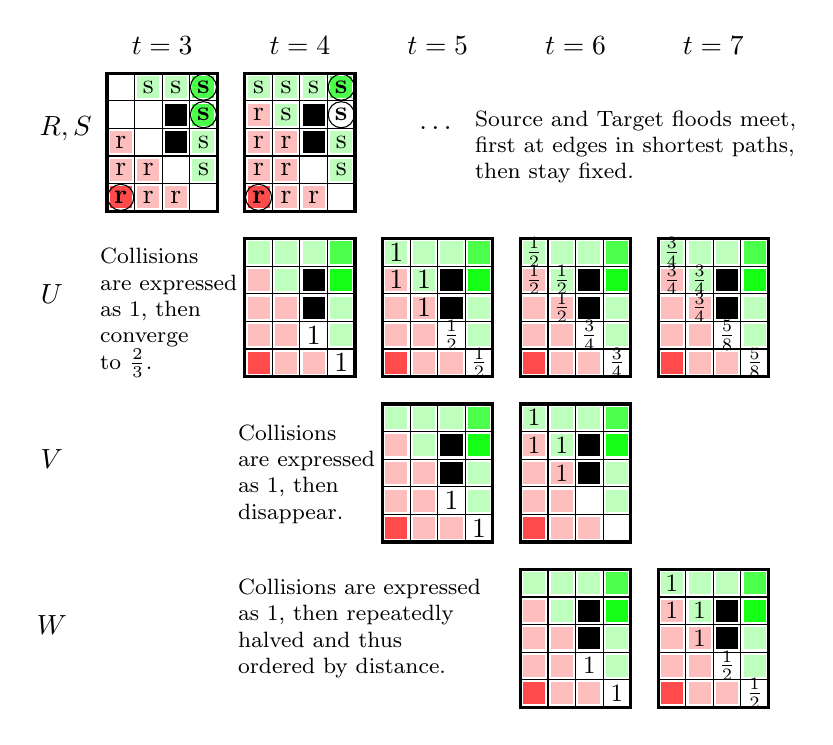
\begin{tikzpicture}[scale=0.7],every node/.style={minimum size=1cm},on grid]
		
    %slanting: production of a set of n 'laminae' to be piled up. N=number of grids.
   %\begin{scope}[
   %        yshift=-83,every node/.append style={
   %        yslant=0.5,xslant=-1},yslant=0.5,xslant=-1
   %        ]
   %    % opacity to prevent graphical interference
   %    \fill[white,fill opacity=0.9] (0,0) rectangle (5,5);
   %    \draw[step=4mm, black] (0,0) grid (5,5); %defining grids
   %    \draw[step=1mm, red!50,thin] (3,1) grid (4,2);  %Nested Grid
   %    \draw[black,very thick] (0,0) rectangle (5,5);%marking borders
   %    \fill[red] (0.05,0.05) rectangle (0.35,0.35);
   %    %Idem as above, for the n-th grid:
   %\end{scope}
	\node[] at (-0.75cm, 1.5cm) {$R , S$};	
	\node[] at (-1cm, -1.5cm) {$U$};	
	\node[] at (-1cm, -4.5cm) {$V$};	
	\node[] at (-1cm, -7.5cm) {$W$};	
	\node[] at (6cm, 1.5cm) {\dots};	
	\node[] at (1, 3){$t=3$};
    \begin{scope}[
    	yshift=0,every node/.append style={
    	    },    	             ]
									 \fill[white,fill opacity=.9] (0,0) rectangle (2,2.5);
									 \draw[black,very thick] (0,0) rectangle (2,2.5);
									 \draw[step=5mm, black] (0,0) grid (2,2.5);
				\fill[red, opacity=0.7] (0.05, 0.05) rectangle ( .45, 0.45);
				\fill[black] (1.05, 1.55) rectangle (1.45, 1.95);
				\fill[black] (1.05, 1.05) rectangle (1.45, 1.45);
				\fill[green, opacity=0.7] (1.55, 2.05) rectangle (1.95, 2.45);
				\node[circle, draw, minimum size = 1] at (0.25, 0.25) {} ;
				\fill[red, opacity=0.25] (0.55, 0.05) rectangle ( .95, 0.45);
				\fill[red, opacity=0.25] (1.05, 0.05) rectangle ( 1.45, 0.45);
				\fill[red, opacity=0.25] (0.55, 0.55) rectangle ( .95, 0.95);
				\fill[red, opacity=0.25] (0.05, 0.55) rectangle ( .45, 0.95);
				\fill[red, opacity=0.25] (0.05, 1.05) rectangle ( .45, 1.45);
				\node[] at (0.25, 0.25) {\bf{r}};
				\node[] at (0.75, 0.75) {r};
				\node[] at (0.75, 0.25) {r};
				\node[] at (0.25, 0.75) {r};
				\node[] at (1.25, 0.25) {r};
				\node[] at (0.25, 1.25) {r};

				\node[circle, draw, minimum size = 1] at (1.75, 2.25) {} ;
				\fill[green, opacity=0.25] (1.05, 2.05) rectangle (1.45, 2.45);
				\fill[green, opacity=0.7] (1.55, 1.55) rectangle (1.95, 1.95);
				\fill[green, opacity=0.25] (1.55, 1.05) rectangle (1.95, 1.45);
				\fill[green, opacity=0.25] (1.55, 0.55) rectangle (1.95, 0.95);
				\fill[green, opacity=0.25] (0.55, 2.05) rectangle (0.95, 2.45);
				\node[circle, draw, minimum size = 1] at (1.75, 1.75) {} ;
				\node[] at (1.75, 2.25) {\bf{s}};
				\node[] at (1.75, 1.75) {\bf{s}};
				\node[] at (1.25, 2.25) {s};
				\node[] at (0.75, 2.25) {s};
				\node[] at (1.75, 1.25) {s};
				\node[] at (1.75, 0.75) {s};
    \end{scope}    	

		\node[] at (3.5, 3){$t=4$};
		\node[] at (6, 3){$t=5$};
		\node[] at (8.5, 3){$t=6$};
		\node[] at (11, 3){$t=7$};
    \begin{scope}[
				yshift=0, xshift=2.5cm,every node/.append style={
    	    },
    	             ]
									 \fill[white,fill opacity=.9] (0,0) rectangle (2,2.5);
									 \draw[black,very thick] (0,0) rectangle (2,2.5);
									 \draw[step=5mm, black] (0,0) grid (2,2.5);
				\fill[red, opacity=0.7] (0.05, 0.05) rectangle ( .45, 0.45);
				\fill[black] (1.05, 1.55) rectangle (1.45, 1.95);
				\fill[black] (1.05, 1.05) rectangle (1.45, 1.45);
				\fill[green, opacity=0.7] (1.55, 2.05) rectangle (1.95, 2.45);
				\node[circle, draw, minimum size = 1] at (0.25, 0.25) {} ;
				\fill[red, opacity=0.25] (0.55, 0.05) rectangle ( .95, 0.45);
				\fill[red, opacity=0.25] (1.05, 0.05) rectangle ( 1.45, 0.45);
				\fill[red, opacity=0.25] (0.55, 0.55) rectangle ( .95, 0.95);
				\fill[red, opacity=0.25] (0.05, 0.55) rectangle ( .45, 0.95);
				\fill[red, opacity=0.25] (0.05, 1.05) rectangle ( .45, 1.45);
				\fill[red, opacity=0.25] (0.05, 1.55) rectangle ( .45, 1.95);
				\fill[red, opacity=0.25] (0.55, 1.05) rectangle ( .95, 1.45);
				\node[] at (0.25, 0.25) {\bf{r}};
				\node[] at (0.75, 0.75) {r};
				\node[] at (0.75, 1.25) {r};
				\node[] at (0.75, 0.25) {r};
				\node[] at (0.25, 0.75) {r};
				\node[] at (1.25, 0.25) {r};
				\node[] at (0.25, 1.25) {r};
				\node[] at (0.25, 1.75) {r};

				\node[circle, draw, minimum size = 1] at (1.75, 2.25) {} ;
				\fill[green, opacity=0.25] (1.05, 2.05) rectangle (1.45, 2.45);
				\fill[green, opacity=0.25] (1.55, 1.05) rectangle (1.95, 1.45);
				\fill[green, opacity=0.25] (1.55, 0.55) rectangle (1.95, 0.95);
				\fill[green, opacity=0.25] (0.55, 2.05) rectangle (0.95, 2.45);
				\fill[green, opacity=0.25] (0.05, 2.05) rectangle (0.45, 2.45);
				\fill[green, opacity=0.25] (0.55, 1.55) rectangle (0.95, 1.95);
				\node[circle, draw, minimum size = 1] at (1.75, 1.75) {} ;
				\node[] at (1.75, 2.25) {\bf{s}};
				\node[] at (1.75, 1.75) {\bf{s}};
				\node[] at (1.25, 2.25) {s};
				\node[] at (0.75, 2.25) {s};
				\node[] at (0.75, 1.75) {s};
				\node[] at (0.25, 2.25) {s};
				\node[] at (1.75, 1.25) {s};
				\node[] at (1.75, 0.75) {s};
    \end{scope}

		
		\begin{scope}[
				yshift=-3cm, xshift=2.5cm,every node/.append style={
    	    },    	             ]
									 \fill[white,fill opacity=.9] (0,0) rectangle (2,2.5);
									 \draw[black,very thick] (0,0) rectangle (2,2.5);
									 \draw[step=5mm, black] (0,0) grid (2,2.5);
				\fill[red, opacity=0.7] (0.05, 0.05) rectangle ( .45, 0.45);
				\fill[red, opacity=0.25] (0.55, 0.05) rectangle ( .95, 0.45);
				\fill[red, opacity=0.25] (1.05, 0.05) rectangle ( 1.45, 0.45);
				\fill[red, opacity=0.25] (0.55, 0.55) rectangle ( .95, 0.95);
				\fill[red, opacity=0.25] (0.05, 0.55) rectangle ( .45, 0.95);
				\fill[red, opacity=0.25] (0.05, 1.05) rectangle ( .45, 1.45);
				\fill[red, opacity=0.25] (0.05, 1.55) rectangle ( .45, 1.95);
				\fill[red, opacity=0.25] (0.55, 1.05) rectangle ( .95, 1.45);
				\fill[black] (1.05, 1.55) rectangle (1.45, 1.95);
				\fill[black] (1.05, 1.05) rectangle (1.45, 1.45);
				\fill[green, opacity=0.7] (1.55, 2.05) rectangle (1.95, 2.45);
				\fill[green, opacity=0.7] (1.55, 1.55) rectangle (1.95, 1.95);
				\fill[green, opacity=0.25] (1.05, 2.05) rectangle (1.45, 2.45);
				\fill[green, opacity=0.7] (1.55, 1.55) rectangle (1.95, 1.95);
				\fill[green, opacity=0.25] (1.55, 1.05) rectangle (1.95, 1.45);
				\fill[green, opacity=0.25] (1.55, 0.55) rectangle (1.95, 0.95);
				\fill[green, opacity=0.25] (0.55, 2.05) rectangle (0.95, 2.45);
				\fill[green, opacity=0.25] (0.05, 2.05) rectangle (0.45, 2.45);
				\fill[green, opacity=0.25] (0.55, 1.55) rectangle (0.95, 1.95);
				\node[] at (1.75, 0.25) {$1$};
				\node[] at (1.25, 0.75) {$1$};
    \end{scope}

    \begin{scope}[
				yshift=-3cm, xshift=5cm,every node/.append style={
				},    	             ]
									 \fill[white,fill opacity=.9] (0,0) rectangle (2,2.5);
									 \draw[black,very thick] (0,0) rectangle (2,2.5);
									 \draw[step=5mm, black] (0,0) grid (2,2.5);
				\fill[red, opacity=0.7] (0.05, 0.05) rectangle ( .45, 0.45);
				\fill[red, opacity=0.25] (0.55, 0.05) rectangle ( .95, 0.45);
				\fill[red, opacity=0.25] (1.05, 0.05) rectangle ( 1.45, 0.45);
				\fill[red, opacity=0.25] (0.55, 0.55) rectangle ( .95, 0.95);
				\fill[red, opacity=0.25] (0.05, 0.55) rectangle ( .45, 0.95);
				\fill[red, opacity=0.25] (0.05, 1.05) rectangle ( .45, 1.45);
				\fill[red, opacity=0.25] (0.05, 1.55) rectangle ( .45, 1.95);
				\fill[red, opacity=0.25] (0.55, 1.05) rectangle ( .95, 1.45);
				\fill[black] (1.05, 1.55) rectangle (1.45, 1.95);
				\fill[black] (1.05, 1.05) rectangle (1.45, 1.45);
				\fill[green, opacity=0.7] (1.55, 2.05) rectangle (1.95, 2.45);
				\fill[green, opacity=0.7] (1.55, 1.55) rectangle (1.95, 1.95);
				\fill[green, opacity=0.25] (1.05, 2.05) rectangle (1.45, 2.45);
				\fill[green, opacity=0.7] (1.55, 1.55) rectangle (1.95, 1.95);
				\fill[green, opacity=0.25] (1.55, 1.05) rectangle (1.95, 1.45);
				\fill[green, opacity=0.25] (1.55, 0.55) rectangle (1.95, 0.95);
				\fill[green, opacity=0.25] (0.55, 2.05) rectangle (0.95, 2.45);
				\fill[green, opacity=0.25] (0.05, 2.05) rectangle (0.45, 2.45);
				\fill[green, opacity=0.25] (0.55, 1.55) rectangle (0.95, 1.95);
				\node[scale=0.9] at (1.75, 0.25) {$\frac{1}{2}$};
				\node[scale=0.9] at (1.25, 0.75) {$\frac{1}{2}$};
				\node[scale=1] at (0.25, 1.75) {$1$};
				\node[scale=1] at (0.25, 2.25) {$1$};
				\node[scale=1] at (0.75, 1.25) {$1$};
				\node[scale=1] at (0.75, 1.75) {$1$};
    \end{scope}

    \begin{scope}[
				yshift=-3cm, xshift=7.5cm,every node/.append style={
				},    	             ]
									 \fill[white,fill opacity=.9] (0,0) rectangle (2,2.5);
									 \draw[black,very thick] (0,0) rectangle (2,2.5);
									 \draw[step=5mm, black] (0,0) grid (2,2.5);
				\fill[red, opacity=0.7] (0.05, 0.05) rectangle ( .45, 0.45);
				\fill[red, opacity=0.25] (0.55, 0.05) rectangle ( .95, 0.45);
				\fill[red, opacity=0.25] (1.05, 0.05) rectangle ( 1.45, 0.45);
				\fill[red, opacity=0.25] (0.55, 0.55) rectangle ( .95, 0.95);
				\fill[red, opacity=0.25] (0.05, 0.55) rectangle ( .45, 0.95);
				\fill[red, opacity=0.25] (0.05, 1.05) rectangle ( .45, 1.45);
				\fill[red, opacity=0.25] (0.05, 1.55) rectangle ( .45, 1.95);
				\fill[red, opacity=0.25] (0.55, 1.05) rectangle ( .95, 1.45);
				\fill[black] (1.05, 1.55) rectangle (1.45, 1.95);
				\fill[black] (1.05, 1.05) rectangle (1.45, 1.45);
				\fill[green, opacity=0.7] (1.55, 2.05) rectangle (1.95, 2.45);
				\fill[green, opacity=0.7] (1.55, 1.55) rectangle (1.95, 1.95);
				\fill[green, opacity=0.25] (1.05, 2.05) rectangle (1.45, 2.45);
				\fill[green, opacity=0.7] (1.55, 1.55) rectangle (1.95, 1.95);
				\fill[green, opacity=0.25] (1.55, 1.05) rectangle (1.95, 1.45);
				\fill[green, opacity=0.25] (1.55, 0.55) rectangle (1.95, 0.95);
				\fill[green, opacity=0.25] (0.55, 2.05) rectangle (0.95, 2.45);
				\fill[green, opacity=0.25] (0.05, 2.05) rectangle (0.45, 2.45);
				\fill[green, opacity=0.25] (0.55, 1.55) rectangle (0.95, 1.95);
				\node[scale=0.9] at (1.75, 0.25) {$\frac{3}{4}$};
				\node[scale=0.9] at (1.25, 0.75) {$\frac{3}{4}$};
				\node[scale=0.9] at (0.25, 1.75) {$\frac{1}{2}$};
				\node[scale=0.9] at (0.25, 2.25) {$\frac{1}{2}$};
				\node[scale=0.9] at (0.75, 1.25) {$\frac{1}{2}$};
				\node[scale=0.9] at (0.75, 1.75) {$\frac{1}{2}$};
    \end{scope}

    \begin{scope}[
				yshift=-3cm, xshift=10cm,every node/.append style={
				},    	             ]
									 \fill[white,fill opacity=.9] (0,0) rectangle (2,2.5);
									 \draw[black,very thick] (0,0) rectangle (2,2.5);
									 \draw[step=5mm, black] (0,0) grid (2,2.5);
				\fill[red, opacity=0.7] (0.05, 0.05) rectangle ( .45, 0.45);
				\fill[red, opacity=0.25] (0.55, 0.05) rectangle ( .95, 0.45);
				\fill[red, opacity=0.25] (1.05, 0.05) rectangle ( 1.45, 0.45);
				\fill[red, opacity=0.25] (0.55, 0.55) rectangle ( .95, 0.95);
				\fill[red, opacity=0.25] (0.05, 0.55) rectangle ( .45, 0.95);
				\fill[red, opacity=0.25] (0.05, 1.05) rectangle ( .45, 1.45);
				\fill[red, opacity=0.25] (0.05, 1.55) rectangle ( .45, 1.95);
				\fill[red, opacity=0.25] (0.55, 1.05) rectangle ( .95, 1.45);
				\fill[black] (1.05, 1.55) rectangle (1.45, 1.95);
				\fill[black] (1.05, 1.05) rectangle (1.45, 1.45);
				\fill[green, opacity=0.7] (1.55, 2.05) rectangle (1.95, 2.45);
				\fill[green, opacity=0.7] (1.55, 1.55) rectangle (1.95, 1.95);
				\fill[green, opacity=0.25] (1.05, 2.05) rectangle (1.45, 2.45);
				\fill[green, opacity=0.7] (1.55, 1.55) rectangle (1.95, 1.95);
				\fill[green, opacity=0.25] (1.55, 1.05) rectangle (1.95, 1.45);
				\fill[green, opacity=0.25] (1.55, 0.55) rectangle (1.95, 0.95);
				\fill[green, opacity=0.25] (0.55, 2.05) rectangle (0.95, 2.45);
				\fill[green, opacity=0.25] (0.05, 2.05) rectangle (0.45, 2.45);
				\fill[green, opacity=0.25] (0.55, 1.55) rectangle (0.95, 1.95);
				\node[scale=0.9] at (1.75, 0.25) {$\frac{5}{8}$};
				\node[scale=0.9] at (1.25, 0.75) {$\frac{5}{8}$};
				\node[scale=0.9] at (0.25, 1.75) {$\frac{3}{4}$};
				\node[scale=0.9] at (0.25, 2.25) {$\frac{3}{4}$};
				\node[scale=0.9] at (0.75, 1.25) {$\frac{3}{4}$};
				\node[scale=0.9] at (0.75, 1.75) {$\frac{3}{4}$};
    \end{scope}




    \begin{scope}[
				yshift=-6cm, xshift=5cm,every node/.append style={
				},    	             ]
									 \fill[white,fill opacity=.9] (0,0) rectangle (2,2.5);
									 \draw[black,very thick] (0,0) rectangle (2,2.5);
									 \draw[step=5mm, black] (0,0) grid (2,2.5);
				\fill[red, opacity=0.7] (0.05, 0.05) rectangle ( .45, 0.45);
				\fill[red, opacity=0.25] (0.55, 0.05) rectangle ( .95, 0.45);
				\fill[red, opacity=0.25] (1.05, 0.05) rectangle ( 1.45, 0.45);
				\fill[red, opacity=0.25] (0.55, 0.55) rectangle ( .95, 0.95);
				\fill[red, opacity=0.25] (0.05, 0.55) rectangle ( .45, 0.95);
				\fill[red, opacity=0.25] (0.05, 1.05) rectangle ( .45, 1.45);
				\fill[red, opacity=0.25] (0.05, 1.55) rectangle ( .45, 1.95);
				\fill[red, opacity=0.25] (0.55, 1.05) rectangle ( .95, 1.45);
				\fill[black] (1.05, 1.55) rectangle (1.45, 1.95);
				\fill[black] (1.05, 1.05) rectangle (1.45, 1.45);
				\fill[green, opacity=0.7] (1.55, 2.05) rectangle (1.95, 2.45);
				\fill[green, opacity=0.7] (1.55, 1.55) rectangle (1.95, 1.95);
				\fill[green, opacity=0.25] (1.05, 2.05) rectangle (1.45, 2.45);
				\fill[green, opacity=0.7] (1.55, 1.55) rectangle (1.95, 1.95);
				\fill[green, opacity=0.25] (1.55, 1.05) rectangle (1.95, 1.45);
				\fill[green, opacity=0.25] (1.55, 0.55) rectangle (1.95, 0.95);
				\fill[green, opacity=0.25] (0.55, 2.05) rectangle (0.95, 2.45);
				\fill[green, opacity=0.25] (0.05, 2.05) rectangle (0.45, 2.45);
				\fill[green, opacity=0.25] (0.55, 1.55) rectangle (0.95, 1.95);
				\node[scale=1] at (1.75, 0.25) {$1$};
				\node[scale=1] at (1.25, 0.75) {$1$};
    \end{scope}

    \begin{scope}[
				yshift=-6cm, xshift=7.5cm,every node/.append style={
				},    	             ]
									 \fill[white,fill opacity=.9] (0,0) rectangle (2,2.5);
									 \draw[black,very thick] (0,0) rectangle (2,2.5);
									 \draw[step=5mm, black] (0,0) grid (2,2.5);
				\fill[red, opacity=0.7] (0.05, 0.05) rectangle ( .45, 0.45);
				\fill[red, opacity=0.25] (0.55, 0.05) rectangle ( .95, 0.45);
				\fill[red, opacity=0.25] (1.05, 0.05) rectangle ( 1.45, 0.45);
				\fill[red, opacity=0.25] (0.55, 0.55) rectangle ( .95, 0.95);
				\fill[red, opacity=0.25] (0.05, 0.55) rectangle ( .45, 0.95);
				\fill[red, opacity=0.25] (0.05, 1.05) rectangle ( .45, 1.45);
				\fill[red, opacity=0.25] (0.05, 1.55) rectangle ( .45, 1.95);
				\fill[red, opacity=0.25] (0.55, 1.05) rectangle ( .95, 1.45);
				\fill[black] (1.05, 1.55) rectangle (1.45, 1.95);
				\fill[black] (1.05, 1.05) rectangle (1.45, 1.45);
				\fill[green, opacity=0.7] (1.55, 2.05) rectangle (1.95, 2.45);
				\fill[green, opacity=0.7] (1.55, 1.55) rectangle (1.95, 1.95);
				\fill[green, opacity=0.25] (1.05, 2.05) rectangle (1.45, 2.45);
				\fill[green, opacity=0.7] (1.55, 1.55) rectangle (1.95, 1.95);
				\fill[green, opacity=0.25] (1.55, 1.05) rectangle (1.95, 1.45);
				\fill[green, opacity=0.25] (1.55, 0.55) rectangle (1.95, 0.95);
				\fill[green, opacity=0.25] (0.55, 2.05) rectangle (0.95, 2.45);
				\fill[green, opacity=0.25] (0.05, 2.05) rectangle (0.45, 2.45);
				\fill[green, opacity=0.25] (0.55, 1.55) rectangle (0.95, 1.95);
				\node[scale=0.9] at (1.75, 0.25) {};
				\node[scale=0.9] at (0.25, 1.75) {$1$};
				\node[scale=0.9] at (0.25, 2.25) {$1$};
				\node[scale=0.9] at (0.75, 1.25) {$1$};
				\node[scale=0.9] at (0.75, 1.75) {$1$};
    \end{scope}


    \begin{scope}[
				yshift=-9cm, xshift=7.5cm,every node/.append style={
				},    	             ]
									 \fill[white,fill opacity=.9] (0,0) rectangle (2,2.5);
									 \draw[black,very thick] (0,0) rectangle (2,2.5);
									 \draw[step=5mm, black] (0,0) grid (2,2.5);
				\fill[red, opacity=0.7] (0.05, 0.05) rectangle ( .45, 0.45);
				\fill[red, opacity=0.25] (0.55, 0.05) rectangle ( .95, 0.45);
				\fill[red, opacity=0.25] (1.05, 0.05) rectangle ( 1.45, 0.45);
				\fill[red, opacity=0.25] (0.55, 0.55) rectangle ( .95, 0.95);
				\fill[red, opacity=0.25] (0.05, 0.55) rectangle ( .45, 0.95);
				\fill[red, opacity=0.25] (0.05, 1.05) rectangle ( .45, 1.45);
				\fill[red, opacity=0.25] (0.05, 1.55) rectangle ( .45, 1.95);
				\fill[red, opacity=0.25] (0.55, 1.05) rectangle ( .95, 1.45);
				\fill[black] (1.05, 1.55) rectangle (1.45, 1.95);
				\fill[black] (1.05, 1.05) rectangle (1.45, 1.45);
				\fill[green, opacity=0.7] (1.55, 2.05) rectangle (1.95, 2.45);
				\fill[green, opacity=0.7] (1.55, 1.55) rectangle (1.95, 1.95);
				\fill[green, opacity=0.25] (1.05, 2.05) rectangle (1.45, 2.45);
				\fill[green, opacity=0.7] (1.55, 1.55) rectangle (1.95, 1.95);
				\fill[green, opacity=0.25] (1.55, 1.05) rectangle (1.95, 1.45);
				\fill[green, opacity=0.25] (1.55, 0.55) rectangle (1.95, 0.95);
				\fill[green, opacity=0.25] (0.55, 2.05) rectangle (0.95, 2.45);
				\fill[green, opacity=0.25] (0.05, 2.05) rectangle (0.45, 2.45);
				\fill[green, opacity=0.25] (0.55, 1.55) rectangle (0.95, 1.95);
				\node[scale=0.9] at (1.75, 0.25) {$1$};
				\node[scale=0.9] at (1.25, 0.75) {$1$};
    \end{scope}

    \begin{scope}[
				yshift=-9cm, xshift=10cm,every node/.append style={
				},    	             ]
									 \fill[white,fill opacity=.9] (0,0) rectangle (2,2.5);
									 \draw[black,very thick] (0,0) rectangle (2,2.5);
									 \draw[step=5mm, black] (0,0) grid (2,2.5);
				\fill[red, opacity=0.7] (0.05, 0.05) rectangle ( .45, 0.45);
				\fill[red, opacity=0.25] (0.55, 0.05) rectangle ( .95, 0.45);
				\fill[red, opacity=0.25] (1.05, 0.05) rectangle ( 1.45, 0.45);
				\fill[red, opacity=0.25] (0.55, 0.55) rectangle ( .95, 0.95);
				\fill[red, opacity=0.25] (0.05, 0.55) rectangle ( .45, 0.95);
				\fill[red, opacity=0.25] (0.05, 1.05) rectangle ( .45, 1.45);
				\fill[red, opacity=0.25] (0.05, 1.55) rectangle ( .45, 1.95);
				\fill[red, opacity=0.25] (0.55, 1.05) rectangle ( .95, 1.45);
				\fill[black] (1.05, 1.55) rectangle (1.45, 1.95);
				\fill[black] (1.05, 1.05) rectangle (1.45, 1.45);
				\fill[green, opacity=0.7] (1.55, 2.05) rectangle (1.95, 2.45);
				\fill[green, opacity=0.7] (1.55, 1.55) rectangle (1.95, 1.95);
				\fill[green, opacity=0.25] (1.05, 2.05) rectangle (1.45, 2.45);
				\fill[green, opacity=0.7] (1.55, 1.55) rectangle (1.95, 1.95);
				\fill[green, opacity=0.25] (1.55, 1.05) rectangle (1.95, 1.45);
				\fill[green, opacity=0.25] (1.55, 0.55) rectangle (1.95, 0.95);
				\fill[green, opacity=0.25] (0.55, 2.05) rectangle (0.95, 2.45);
				\fill[green, opacity=0.25] (0.05, 2.05) rectangle (0.45, 2.45);
				\fill[green, opacity=0.25] (0.55, 1.55) rectangle (0.95, 1.95);
				\node[scale=0.9] at (0.25, 1.75) {$1$};
				\node[scale=0.9] at (0.25, 2.25) {$1$};
				\node[scale=0.9] at (0.75, 1.25) {$1$};
				\node[scale=0.9] at (0.75, 1.75) {$1$};
				\node[scale=0.9] at (1.75, 0.25) {$\frac{1}{2}$};
				\node[scale=0.9] at (1.25, 0.75) {$\frac{1}{2}$};
    \end{scope}

\tikzset{story/.style={font=\footnotesize, anchor=north west, align=left}}
\node[story] at (6.5, 2) {Source and Target floods meet,\\first at edges in shortest paths,\\
 then stay fixed.};

\node[story] at (-0.3, -0.5) {Collisions \\are expressed\\as $1$, then\\converge\\to $\frac{2}{3}$.};
\node[story] at (2.2, -3.7) {Collisions \\are expressed\\as $1$, then\\disappear.};
\node[story] at (2.2, -6.5) {Collisions are expressed \\as $1$, then  repeatedly\\ halved and thus\\ ordered  by distance.};

\end{tikzpicture}

\end{frame}
\begin{frame}
\pgfplotsset{every axis plot/.append style={each nth point=1}}
\pgfplotsset{possible/.style={dashed, thick, samples=100, color =PineGreen}}
\pgfplotsset{width=13cm, height=4cm}
\begin{tikzpicture}[every mark/.append style={mark size=1.5pt}]
    \pgfmathsetlengthmacro\MajorTickLength{\pgfkeysvalueof{/pgfplots/major tick length} * 2
		}
  \begin{axis}[domain  = -21:35,
         axis x line = center,
         axis y line = center,
         samples = 100,
         xmin    = -20,
         xmax    = 36,
         ymin    = -.5,
         ymax    = 1.5,
         xtick={},
         ytick={1},
         xtick   = {-20, -16, -12, -8, -4, 0, 1, 6, 12, 18, 23, 26, 29, 32},
         xlabel  = {$a$},
         ylabel  = {$g(a)$},
         set layers,
         every axis plot/.append style={blue},
         x label style={
             anchor=west,},
         y label style={
             anchor=south,
         },
         major tick length = \MajorTickLength,
         every tick/.style={
         black,
     semithick,},
         minor tick num = 4,
         legend cell align=left,
         legend style={fill=white, 
             fill opacity=0.6, text opacity=1, draw=none, font=\footnotesize,
             at={(-.05,1.3,0)}, anchor=north west},
         grid = both,
               ]
							\addplot[domain= -23:0, possible] {0};
							\addplot[domain= 0:1, possible, forget plot] {x};
				\addplot[possible, domain= 1:5, forget plot] coordinates{
			(1, 1)
			(2, 1)
			(3, 1)
			(4, 1)
			(5, 1)
			(6, 0) (7, 1) (11, 1) 
			(12, 0) (13, 1) (17, 1) 
			(18, 0) (19, 1)
			(20, 1)
			(35, 1)
	};
							 \addplot[samples=100, only marks, domain=-20:0, mark=*, opacity=0.5] coordinates{
							 (-20, 0) 
						   (-16, 0) 
							 (-15, 0) 
						   (-12, 0) (-11, 0) 
						(-10, 0) 
					(-8, 0) (-7, 0) (-6, 0) (-5, 0) 
				(-4, 0) (-3, 0) (-2, 0) (-1, 0) (0, 0)
			(20,1)
			(23, 1)
			(24, 1)
			(26, 1)
			(27, 1) (28, 1)
			(29, 1)
			(30, 1) (31, 1) 
			(32, 1)
			(33, 1) (34, 1) (35, 1) (36, 1)

			(1, 1)
			(2, 1)
			(3, 1)
			(4, 1)
			};

	\addplot[only marks, color=red, opacity=0.5, samples=100, domain= 1:5, mark=*] coordinates{
		(-6,0) (-5, 0) (-4, 0) (-3,-0) (-2, 0) (-1,0)
		(0,0) 
			(1, 1)
			(2, 1)
			(3, 1)
			(4, 1)
			(6, 0) (7, 1) (8, 1) (9, 1) 
			(12, 0) (13, 1) (14, 1)
			(18, 0) (19, 1)
			(1/2, 1/2)
					(3/4, 3/4)
					(5/8, 5/8)
					(11/16, 11/16)
					(21/32, 21/32)
					(43/64, 43/63)
	};
				\addplot[only marks, samples=100, domain= 0:1, color=green!50!gray, opacity=0.5] coordinates{
					(1, 1)
					(1/2, 1/2)
					(1/4, 1/4)
					(1/8, 1/8)
					(1/16, 1/16)
					(1/32, 1/32)
					(1/64, 1/64)
					(1/128, 1/128)
					(1/256, 1/256)
					(1/512, 1/512)

	};
\addlegendentry{possible nonlinearity $g(a)$}
\addlegendentry{activations in $R$ and $S$}
\addlegendentry{'' in channel $U$}
\addlegendentry{'' in $W$}
\end{axis}
\end{tikzpicture}
\begin{columns}
    \begin{column}{0.7\linewidth}
Like the "physarum" slime mould (which has been modeled as a CA), the CA pathfinding algorithm finds shortest paths by sending out floods of activation from sources and targets. Once the floods meet:
\begin{outline}
    \1 In "physarum," the spread continues for some time, before longer paths are pruned.
    \1 In our CA, the timestep of first contact between the floods is recorded at each tile.
\end{outline}
    \end{column}
    \begin{column}{0.3\linewidth}
\includegraphics[width=\linewidth]{images/slimeMould.jpg}
    \end{column}
\end{columns}
\end{frame}


%\begin{frame}
%Something that plays a game, or manages some simulation, on a small map, should be expected to do the same on a larger map.
%
%As long as the game, or simulation-rules, can exist naturally at variable scales, then so should our agent's understanding of them, with little or no additional learning.
%
%Representation of the game should be map-size invariant.
%
%We want an agent that:
%\begin{itemize}
%	\item considers the entire gameboard at each step, and can act anywhere on the gameboard at each step; and 
%	\item whose every action can result from any observation.
%\end{itemize}
%Even a small window manoeuvered across a larger board should be scalable.
%\end{frame}

\section{Conclusion}

\begin{frame}
    In the POET (Paired Open-Ended Trailblazer) algorithm, the environment is mutated incrementally in order to challenge the agent to develop a diverse set of gameplay strategies.

    \begin{outline}
    \1 Our next step: use POET to mutate a target vector (or reward-weight vector) to encourage the agent to become adept in developing cities with different overall character.
        \2 The player will be able to control this target vector in real-time, modifying the agent's behaviour at a high-level.
    \end{outline}
\end{frame}

\begin{frame}
	Recent work has leveraged intrinsic curiosity to train RL agents to generate ``life'' in Lenia, a continuous-valued adaptation of Conway's Game of Life.
\begin{outline}
	\1 A CPPN generates starting configurations.
	\1 A VAE attempts to predict the resulting activity of the simulation.
		\2 Its hidden activation-space is treated as the CPPN's goal-space.
\end{outline}
	Algorithm:
\begin{outline}
    \1 The CPPN is evolved to elicit the target vector in the VAE 
    \1 The target is sampled uniformly from a sufficiently large hyupercube in goal-space
\end{outline}
    Note that the agent provides only the initial state (rather than acting on each tick), and affects all tiles at once (rather than one at a time).
\end{frame}
\begin{frame}
	Proposal: Agent and Environment emerge from same substrate, and co-evolve, driven by instrinsic curiosity.
\end{frame}

\begin{frame}
    \frametitle{Summary}
    \begin{outline}
        \1 New RL environments: SimCity, (step-wise interactive) Game of Life, and a minimal but challenging pathfinding problem.
            \2 Inherently open-ended (SC and GoL). Interactive.
            \2 Variable map-sizes.
        \1 Weight-sharing in FNNs allows for 0-shot transfer to larger map-sizes with the possibility for global policies.
        \1 A new fractal expansion rule saves compute when scaling up, while encouraging dimensionality reduction.
            \2 Conjecture: in addition to their form and function, these FNNs possess fractal representations of the map (and produce fractal structures upon it over time).
        \1 A NN implementation of a CA pathfinding algorithm.
            \2 A possible path toward a general mapping from CA to NN.
            \2 A possible paradigm for the co-evolution of game-player and game-mechanics.
    \end{outline}
\end{frame}

\end{document}
